\section{Lidar detection range analysis}
It is useful to know possible range of detection based on lidar sensor. This range influences the way how the waypoints for exploration are generated. Higher the detection range is, lower number of waypoints is necessary for exploring whole arena. There is a limited time for exploration, because brick pickup and brick placement takes a lot of time. Speed of pickup and placement is limited mainly by the speed of Kinova arm. We estimate the maximal range using the figure \ref{fig:range}.

\begin{figure}[H]
\centering
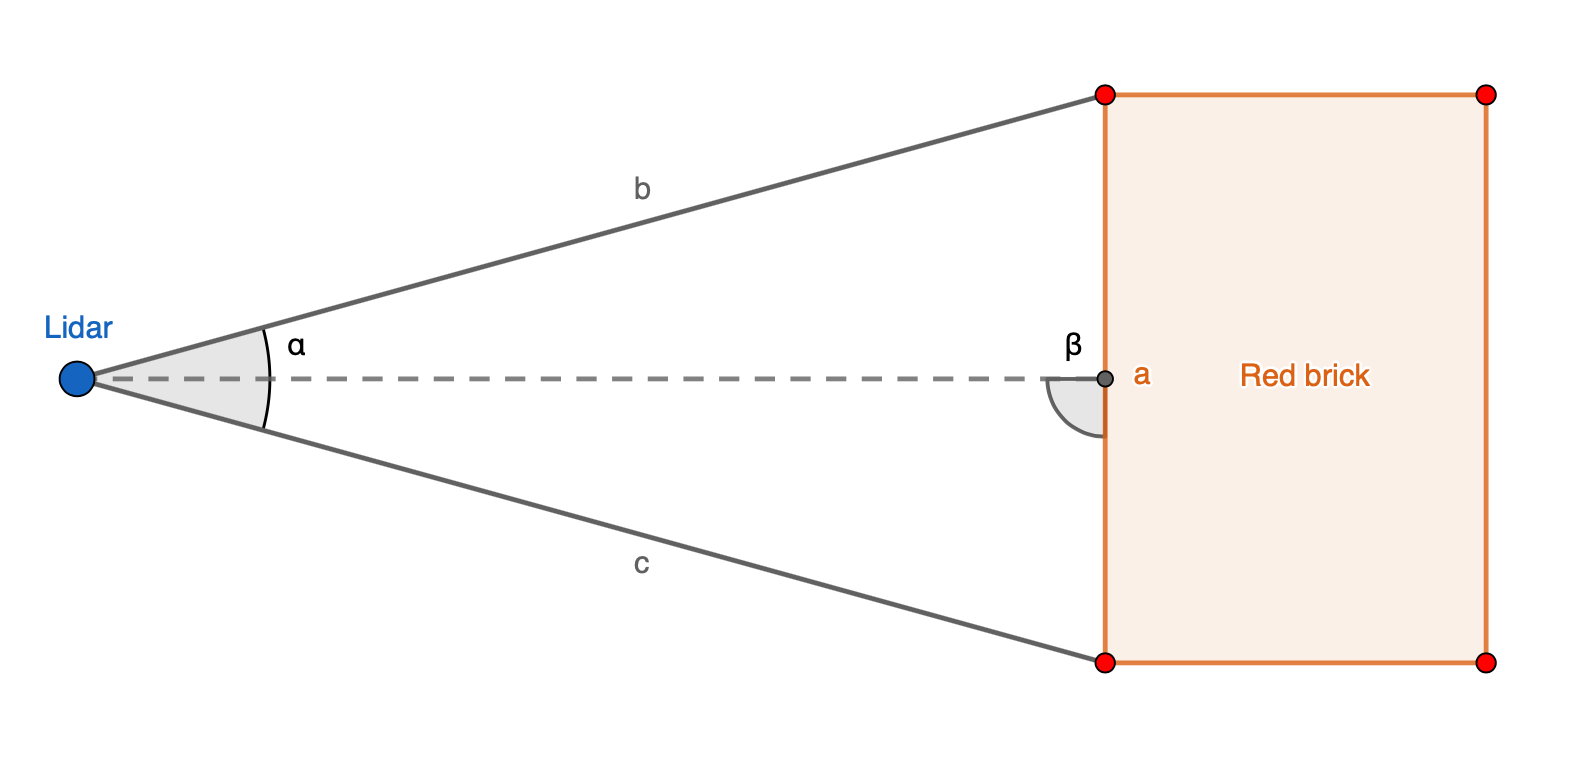
\includegraphics[scale=1.1]{fig/lidar_range.png}
\caption[Lidar range study]{Visualization of rays hitting the red brick.}
\label{fig:range}
\end{figure}

Angle $\alpha$ is the resolution of lidar known from table \ref{tab:lidar}. Only the maximal range is calculated thus angle $\beta = 90\degree$. To obtain the distance between points on the brick the cosine theorem can be used.
\begin{equation}
a^2 = b^2 + c^2 - 2bc \cos \alpha.
\end{equation}
Because $\beta$ is right angle we can write $b = c$ and thus:
\begin{equation}
a = \sqrt{2b^2 \left(1-\cos \alpha \right)}.
\end{equation}
Now we want to know how many rays $N$ would hit the brick from given distance $b$ with lidar angular resolution $\alpha$ and size of the brick $a$. 
\begin{align}
a &= \sqrt{2b^2 \left(1-\cos \left( N \alpha \right) \right)} \\
N &= \frac{\arccos\left(1-\frac{a^2}{2b^2}\right) }{\alpha}
\label{eq:rays}
\end{align}
Finally we can plot a function of number of rays $N$ with respect to distance to object $b$. This analysis can be done similarly for vertical and horizontal resolution.

\begin{figure}[H]
\centering
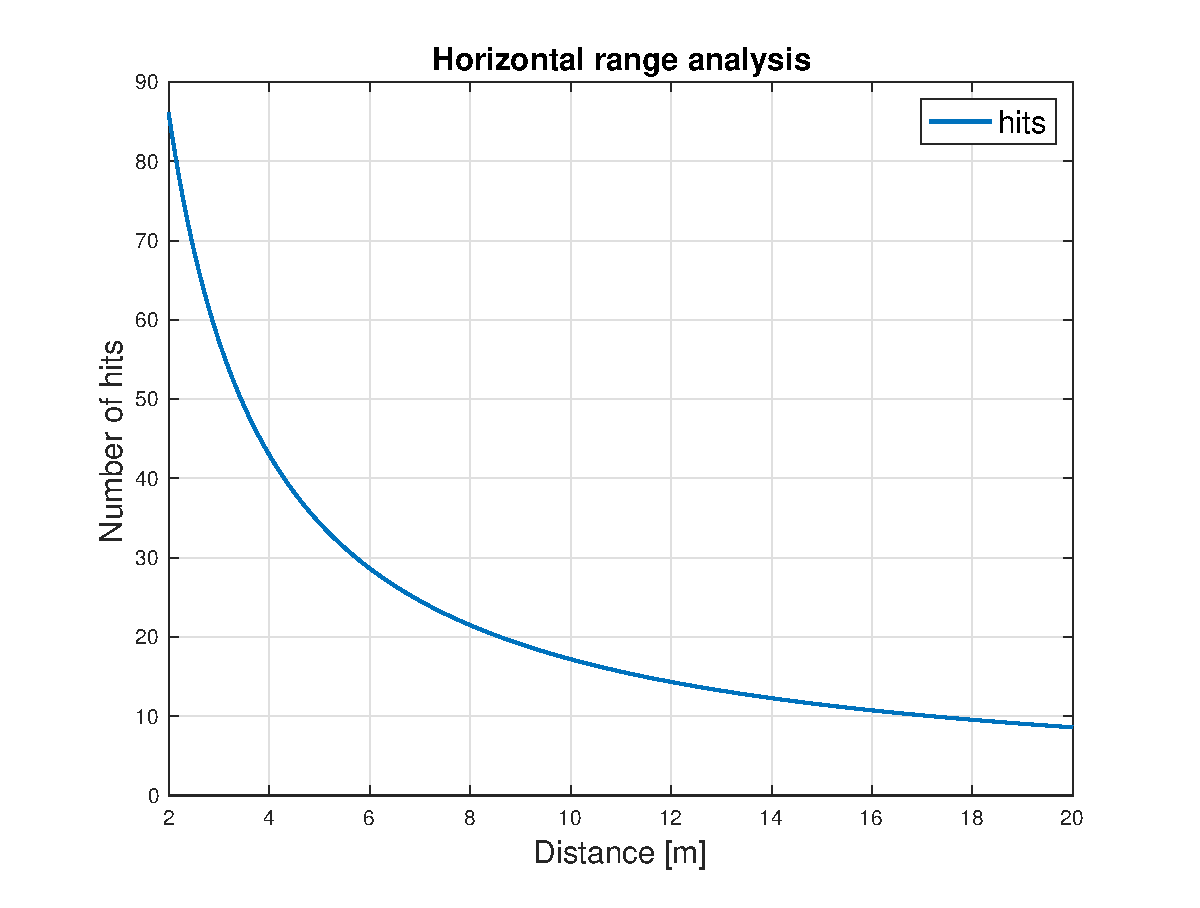
\includegraphics[scale=0.5]{fig/horizontal_range.eps}
\caption[Horizontal range chart]{Number of hits of the smallest brick from given distance.}
\label{fig:horizontal_hits}
\end{figure}

In the figure \ref{fig:horizontal_hits} is clearly visible that the horizontal resolution of the lidar is not limiting factor of the range. Even from 10 meters is lidar able to hit red brick more than 15 times. On the other hand the figure \ref{fig:vertical_hits} shows that pile of bricks with height 40 cm would be hit by less than two lidar layers from distance bigger than 6 meters. Furthermore this is the best case scenario analysis where $\beta$ is right angle which happens rarely in reality.
 
\begin{figure}[H]
\centering
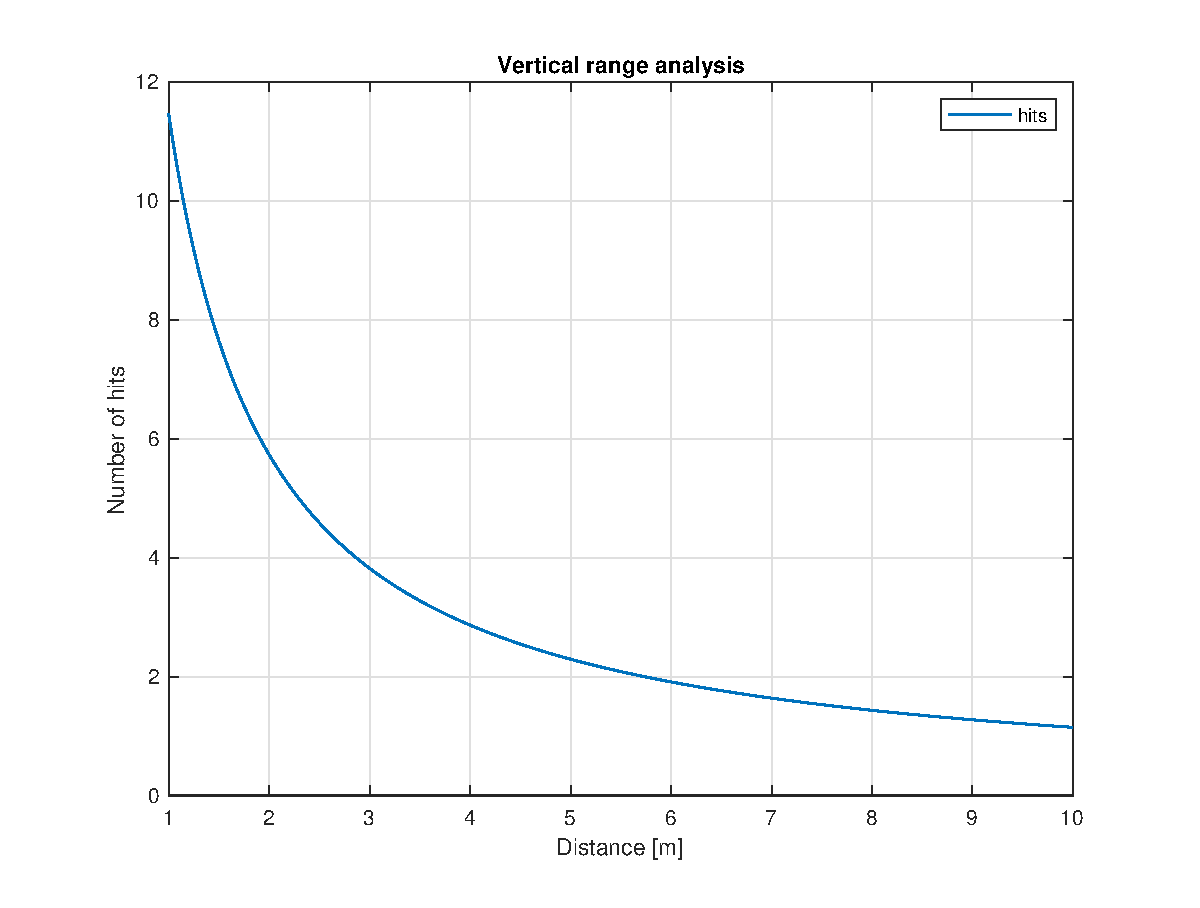
\includegraphics[scale=0.5]{fig/vertical_range.eps}
\caption[Horizontal range chart]{Number of hits of two stacked bricks from given distance.}
\label{fig:vertical_hits}
\end{figure}




\section{Detection pipeline}

\subsection{Line segmentation}

\subsection{Pile detection}

\subsection{Pattern fitting}
